\documentclass[a4paper]{scrreprt}

\usepackage{url}
\usepackage{graphicx}

\begin{document}

\title{BPMN 2.0 Editor\\-- Installation Guide --}
\author{Marcel Michel}

\maketitle

%\tableofcontents

\chapter{BPMN 2.0 Editor}

\section{Requirements}
\begin{itemize}
	\item Eclipse 3.6 (Helios) or newer
	\item Graphiti framework. \\Update site: \url{http://download.eclipse.org/graphiti/updates/0.7.1/}
	\item Eclipse Modeling Framework
\end{itemize}

\section{Installation}
There are two possibilities to get the latest editor version:

\subsection{Using update site}
Use \url{http://codehoop.com/bpmn2} update site (Figure \ref{fig:updatesite.png}).\\ \\
\begin{figure}
	\centering	
	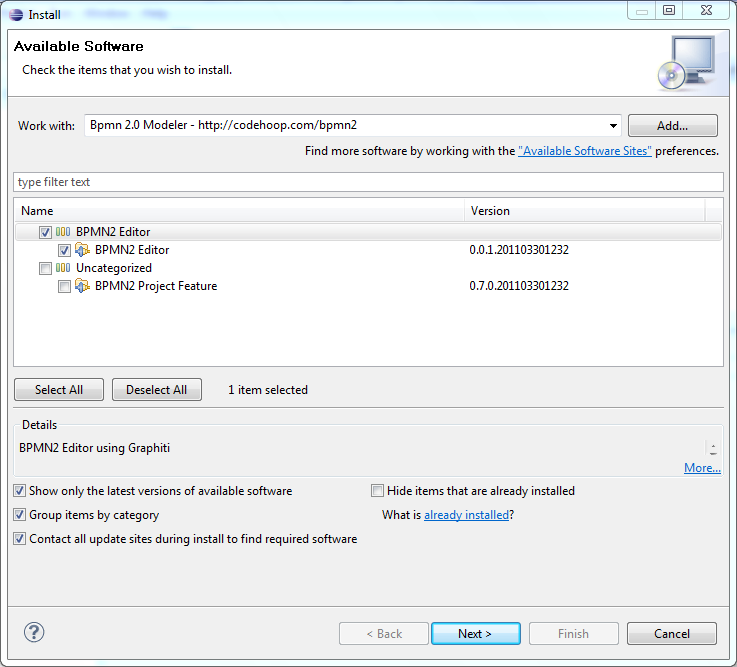
\includegraphics[scale=0.5]{images/updatesite.png}
	\caption{Update site}
	\label{fig:updatesite.png}
\end{figure}
\textbf{Note:} The Feature project includes the bpmn2 metamodel, so select it if you have not currently installed the bpmn2 metamodel. 

\subsection{Using GIT}
If you want to run the editor from source you also need to check out the source project of the bpmn2 metamodel at \url{http://git.eclipse.org/c/bpmn2/}.

Use \url{git://github.com/imeikas/BPMN2-Editor-for-Eclipse.git} to get the source version of the editor.

\subsection{Appendix}
For further information please visit the following websites:
\begin{itemize}
	\item BPMN 2.0 Editor Wiki \\ \url{https://github.com/imeikas/BPMN2-Editor-for-Eclipse/wiki}
	\item BPMN 2.0 Modeler - Proposal \\ \url{http://www.eclipse.org/proposals/soa.bpmn2-modeler/}
\end{itemize}

\begin{figure}
	\centering	
	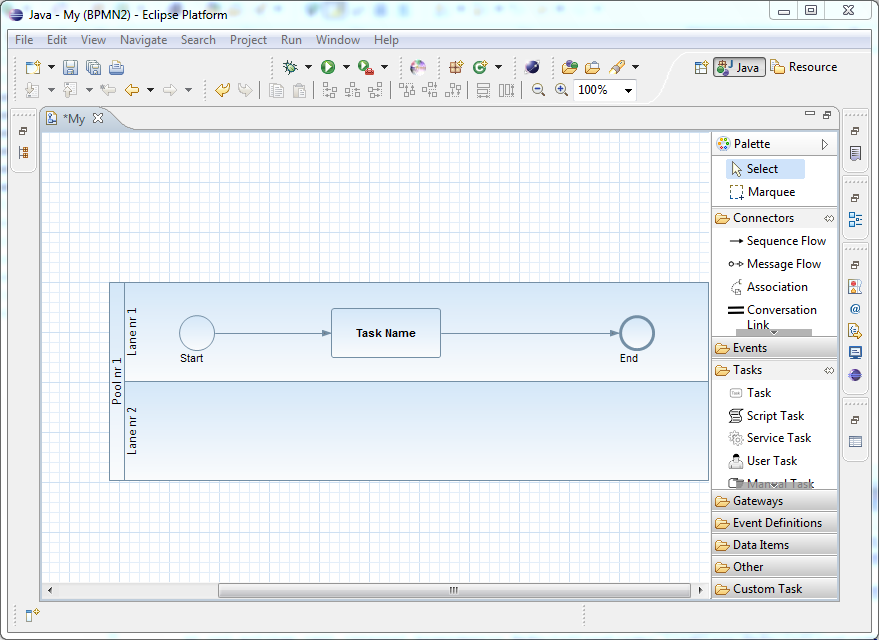
\includegraphics[scale=0.5]{images/modeler.png}
	\caption{The BPMN 2.0 Modeler}
	\label{fig:modeler.png}
\end{figure}

\end{document}
